\documentclass{article}
\title{Intro to PDEs: Ch 2.1 HW}
\author{Logan Rhyne, Harley Combest, Roy Galang}
\usepackage[T1]{fontenc}
\usepackage{amsfonts, amsmath, amsthm, amssymb}
\usepackage{mathtools, bigints, empheq}
\usepackage{graphicx, wrapfig, xcolor, float}
\usepackage{stackrel}
\usepackage{pgfplots}
\usepackage[shortlabels]{enumitem}
\usepackage[margin=1.0in]{geometry}
\setlength{\parindent}{0pt}
\theoremstyle{definition}
\newtheorem*{lemma}{Lemma}
\newtheorem*{conj}{Conjecture}
\newtheorem{prob}{}
\newtheorem*{pf}{Proof}
\newtheorem*{dpf}{Disproof}
\renewcommand\qedsymbol{$\blacksquare$}
\renewcommand{\emptyset}{\varnothing}
\renewcommand{\epsilon}{\varepsilon}
\newenvironment{disproof}{\begin{proof}[Disproof]}{\end{proof}}
\newenvironment{ans}{\begin{proof}[Answer]\renewcommand{\qedsymbol}{}}{\end{proof}}
\newenvironment{boldenv}{\bfseries\boldmath}{}
\newcommand{\N}{\mathbb{N}}
\newcommand{\Z}{\mathbb{Z}}
\newcommand{\R}{\mathbb{R}}

\pgfplotsset{compat=1.18}

\DeclareMathOperator{\ran}{range}

\begin{document}
	
	\maketitle
	
	\begin{boldenv}
		\underline{Problem 1}. Consider each of the following equations.
            \begin{enumerate}[(1), series=problems]
			\item $2u_t + 3u_x = 0$
			\item $u_t + tu_x = 0$
			\item $u_t - tu_x = 0$
			\item $u_t + t^2u_x = 0$
			\item $u_t + xu_x = 0$
			\item $u_t + txu_x = 0$
                \item $u_t + x^2u_x = 0$
			\item $u_t + (x^2+1)u_x = 0$
			\item $u_t + (t^2+1)u_x = 0$
			\item $(x+1)u_t + u_x = 0$
			\item $(x+1)^2u_t + u_x = 0$
            \item $(x^2+1)u_t + u_x = 0$
            \item $(x^2-1)u_t + u_x = 0$
		\end{enumerate}
            \begin{enumerate}[(a), leftmargin=4em]
                \item Draw characteristics and find the general solution $u=u(t,x)$ for each equation.
                \item For each problem, consider the IVP  $u(0,x) = f(x)$ for $x \in \R$. Does the solution always exist? If not, what conditions should $f(x)$ satisfy? Consider the solution for both $t>0$ and $t<0$ separately. 
                \item Where is the solution is uniquely determined? Consider separately $t>0$ and $t<0$.
                \item For the cases $\{ t>0, x>0 \}$ and $\{ t>0, x<0 \}$ with initial condition $u(0,x) = f(x)$, are the solutions defined everywhere?  Do we need to impose a condition at $x=0$, i.e. do we need to impose $u(t,0) = g(t)$? If so, solve the IBVP. 
                \item Consider the previous sub-problem for $t<0$.
            \end{enumerate}
            
                
            \end{boldenv}
	{\color{red} For each of these problems, when you plug in the initial condition you should obtain $f(x)$ or $g(t)$ in general , you really shouldn't be plugging in the same condition when you have boundary conditions. You should clean this up to reflect this, the constant $C$ really represents where you are starting your characteristic curve either $(x_{0},0)$ or $(0,t_{0})$ respectively, In certain instances this doesn't quite effect the nature of the solution. But these types of problems are more intricate then just plugging in the constant of integration you obtain. The entire process, is use using one of the variables as a parameter, and effectively solving an ODE in one-variable. So in the former case, we know that along characteristics emanating from $(x_{0},0)$ 
    $$
    u(t,x) = u(t,x(t)) =^{!} u(0,x_{0}) = f(x_{0}). 
    $$ 
    Here in a since you need the $x_{0}$ where the curve begins. This would be similar when assigning data at $x=0$. Most of these solutions in fact start at scaled version of the function. 
 }	
	
	\begin{ans}
		\begin{enumerate}[(1), series=answers]
			
			\item \begin{enumerate}[a)]
                    \item Using the method of characteristics, we can use the integral curves to get
                    \begin{align*}
                        \frac{dt}{2} &= \frac{dx}{3}\\
                        \frac{t}{2} &= \frac{x}{3} + C\\
                        \frac{t}{2} - \frac{x}{3} &= C\\
                    \end{align*}
                    We will assume an initial condition $u(x,0) = f(x)$. This would mean that the function is constant along the characteristic curves $u(x,t)=f(C)$. For this PDE, the solution is $\boxed{u(x,t)=f\left(\frac{t}{2} - \frac{x}{3}\right)}$. Its characteristic curves are shown below:

                    \begin{center}
                    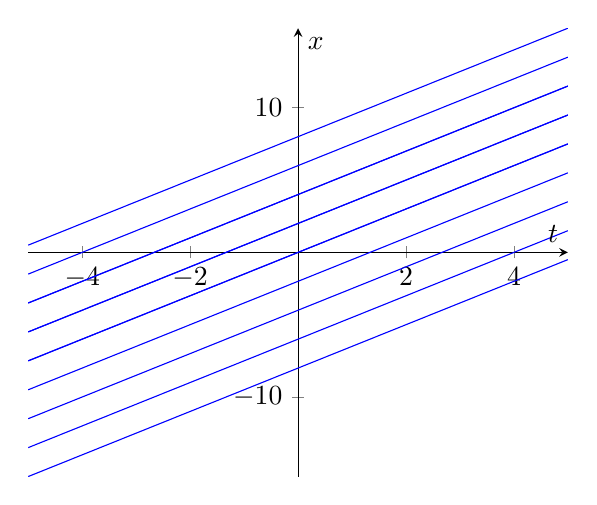
\begin{tikzpicture}
                    \begin{axis}[axis lines = middle, xlabel=$t$, ylabel=$x$]
                    
                    \foreach \C in {-8, -6,...,0,..., 6, 8} {
                    \addplot[color=blue]{3*x/2 - \C};
                    }
                        
                    \end{axis}
                    \end{tikzpicture}
                    \end{center}

                    \item For both cases of $t > 0$ and $t < 0$ for $-\infty < x < \infty$, there will always be a solution.

                    \item For both cases of $t > 0$ and $t < 0$, the solution is uniquely determined.

                    \item Assuming there is an initial condition $u(0,x) = f(x)$:\\
                    \underline{$t > 0, x > 0$}: As we have restricted ourselves to Quadrant I, we can see that we need to put a condition when $x < \frac{3t}{2}$. Taking $u(t,0) = g(t)$, 
                    \begin{equation*}
                    u(x,t) =
                    \begin{cases}
                        f\left(\frac{t}{2}-\frac{x}{3}\right), & x > \frac{3t}{2}\\
                        g\left(\frac{t}{2}-\frac{x}{3}\right), & x < \frac{3t}{2}
                    \end{cases}
                    \end{equation*}\\
                    \underline{$t > 0, x < 0$}: Solutions are defined everywhere in this quadrant.

                    \item \underline{$t < 0, x > 0$}: By symmetry, the solutions in this quadrant are defined everywhere.\\
                    \underline{$t < 0, x < 0$}: By symmetry, we need another condition (which is the same as for the case in Quadrant I) for the Quadrant III. The only difference is that we must now consider $x > \frac{3t}{2}$.
                \end{enumerate}
			
			\item \begin{enumerate}[a)]
                    \item Using the method of characteristics, we get the following:
                    \begin{align*}
                        \frac{dt}{1} &= \frac{dx}{t}\\
                        \int t\,dt &= \int dx\\
                        \frac{1}{2}t^2 &= x+C\\
                        \frac{1}{2}t^2 -x &= C\\
                    \end{align*}
                    If we assume an initial condition $u(x,0) = f(x)$, then since the function is constant along characteristic curves, we have that $\boxed{u(x,t) = f(C) = f\left(\frac{1}{2}t^2 - x\right)}$. It has the following characteristic curves:
                    
                    \begin{center}
                    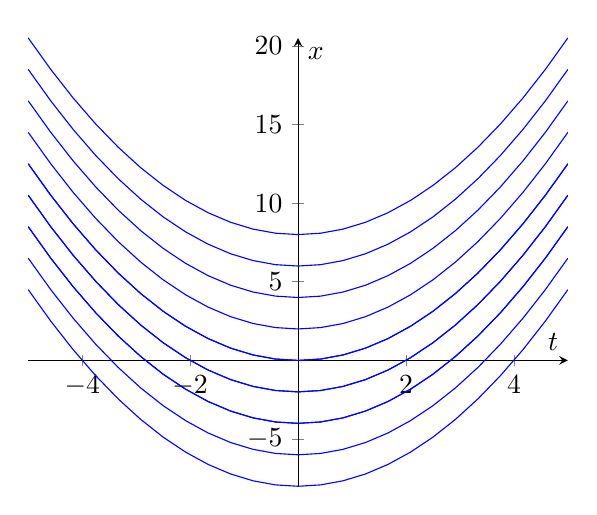
\begin{tikzpicture}
                    \begin{axis}[axis lines = middle, xlabel=$t$, ylabel=$x$]
                    
                    \foreach \C in {-8, -6,...,0,..., 6, 8} {
                    \addplot[color=blue]{x^2/2 + \C};
                    }
                    \end{axis}
                    \end{tikzpicture}
                    \end{center}
                    
                    \item For each case of $t > 0$ and $t < 0$, a solution always exists.

                    \item The solution is uniquely determined everywhere it exists.

                    \item \underline{$t > 0, x > 0$}: Since we are only considering the upper-right quadrant, we must impose a condition $u(0,t) = g(t)$ when $x < \frac{1}{2}t^2$. We also have that $u(x,t) = g(C)$. Taking $f(0) = g(0)$ and $f,g\in C^1$, we have our overall solution that
                    \begin{equation*}
                    u(x,t) =
                    \begin{cases}
                        f\left(\frac{1}{2}t^2 - x\right), & x > \frac{1}{2}t^2\\
                        g\left(\frac{1}{2}t^2 - x\right), & x < \frac{1}{2}t^2
                    \end{cases}
                    \end{equation*}
                    \underline{$t > 0, x < 0$}: There is a solution defined everywhere.

                    \item \underline{$t < 0, x > 0$}: By symmetry, the conditions are the same as when $t > 0, x > 0$.
                    
                    \underline{$t < 0, x < 0$}: By symmetry, there is a solution defined everywhere, as in $t > 0, x < 0$.
                \end{enumerate}
			
			\item \begin{enumerate}[a)]
                    \item Using the method of characteristics, we get the following: 
				\begin{align*}
					\frac{dt}{1} &= -\frac{dx}{t}\\
					\int t\, dt &= -\int dx\\
					\frac{t^2}{2} &= -x + C\\
				\end{align*}
			If we assume an initial condition $u(x, 0) = f(x)$, then, since the function is constant along characteristic curves, we have that $\boxed{u(x, t) = f(C) = f(\frac{t^2}{2} + x)}$. It has the following characteristic curves:

                    \begin{center}
                    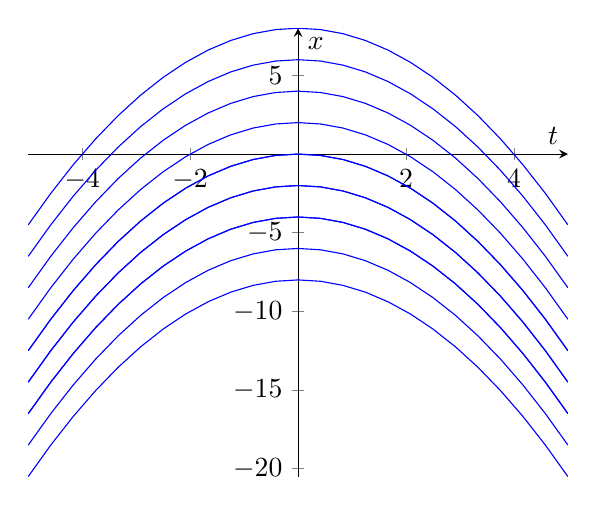
\begin{tikzpicture}
                    \begin{axis}[axis lines = middle, xlabel=$t$, ylabel=$x$]
                    
                    \foreach \C in {-8, -6,...,0,..., 6, 8} {
                    \addplot[color=blue]{\C - x^2/2};
                    }
                    \end{axis}
                    \end{tikzpicture}
                    \end{center}
                    
                    \item For each case of $t > 0$ and $t < 0$, a solution always exists.

                    \item The solution is uniquely determined everywhere it exists.

                    \item For $x < 0$, need $u(t, 0) = g(t)$ when $0 > x \geq - \frac{t^2}{2}$ and $f(0) = g(0)$

                    \item See (d).

                \end{enumerate}
			
			\item \begin{enumerate}[a)]
                    \item Using the method of characteristics, we get the following:
                    \begin{align*}
                        \frac{dt}{1} &= \frac{dx}{t^2}\\
                        \int t^2\,dt &= \int dx\\
                        \frac{1}{3}t^3 &= x+C\\
                        \frac{1}{2}t^2 -x &= C\\
                    \end{align*}
                    If we assume an initial condition $u(x,0) = f(x)$, then since the function is constant along characteristic curves, we have that $\boxed{u(x,t) = f(C) = f\left(\frac{1}{3}t^3 - x\right)}$. It has the following characteristic curves:
                    
                    \begin{center}
                    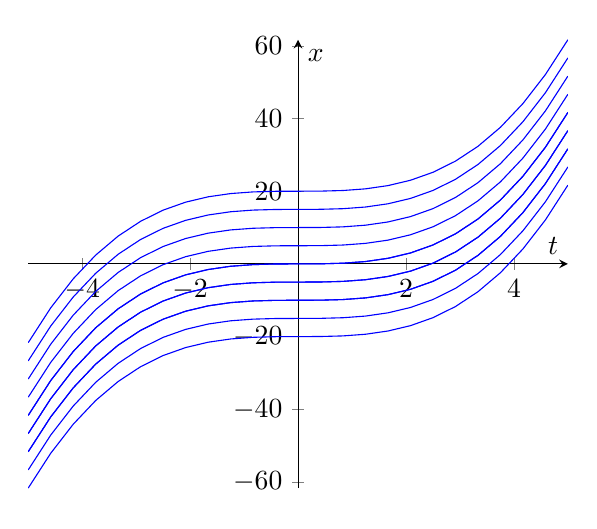
\begin{tikzpicture}
                    \begin{axis}[axis lines = middle, xlabel=$t$, ylabel=$x$]
                    
                    \foreach \C in {-20, -15,...,0,..., 15, 20}
                    {
                    \addplot[color=blue]{x^3/3 + \C};
                    }
                    \end{axis}
                    \end{tikzpicture}
                    \end{center}
                    
                    \item For each case of $t > 0$ and $t < 0$, a solution always exists.

                    \item The solution is uniquely determined everywhere it exists.

                    \item \underline{$t > 0, x > 0$}: Since we are only considering the upper-right quadrant, we must impose a condition $u(0,t) = g(t)$ when $x < \frac{1}{3}t^3$. We also have that $u(x,t) = g(C)$. Taking $f(0) = g(0)$ and $f,g\in C^1$, we have our overall solution that
                    \begin{equation*}
                    u(x,t) =
                    \begin{cases}
                        f\left(\frac{1}{3}t^3 - x\right), & x > \frac{1}{3}t^3\\
                        g\left(\frac{1}{3}t^3 - x\right), & x < \frac{1}{3}t^3
                    \end{cases}
                    \end{equation*}
                    \underline{$t > 0, x < 0$}: There is a solution defined everywhere.

                    \item \underline{$t < 0, x > 0$}: By symmetry, the conditions are similar to when $t > 0, x > 0$, only with the bounds of each piecewise part reversed, resulting in  \begin{equation*}
                    u(x,t) =
                    \begin{cases}
                        f\left(\frac{1}{3}t^3 - x\right), & x < \frac{1}{3}t^3\\
                        g\left(\frac{1}{3}t^3 - x\right), & x > \frac{1}{3}t^3
                    \end{cases}
                    \end{equation*}
                    
                    \underline{$t < 0, x < 0$}: By symmetry, there is a solution defined everywhere, as in $t > 0, x < 0$.
                \end{enumerate}
			
			\item \begin{enumerate}[a)]
                    \item Using the method of characteristics, we get the following:
                    \begin{align*}
                        \frac{dt}{1} = \frac{dx}{x}\\
                        t=\ln(\frac{x}{C})\\
                        Ce^t = x\\
			C = xe^{-t}
                    \end{align*}
                    If we assume an initial condition $u(x,0) = f(x)$, then since the function is constant along characteristic curves, we have that $\boxed{u(x,t) = f(C) = f\left(xe^{-t}\right)}$. It has the following characteristic curves:
                    
                    \begin{center}
                    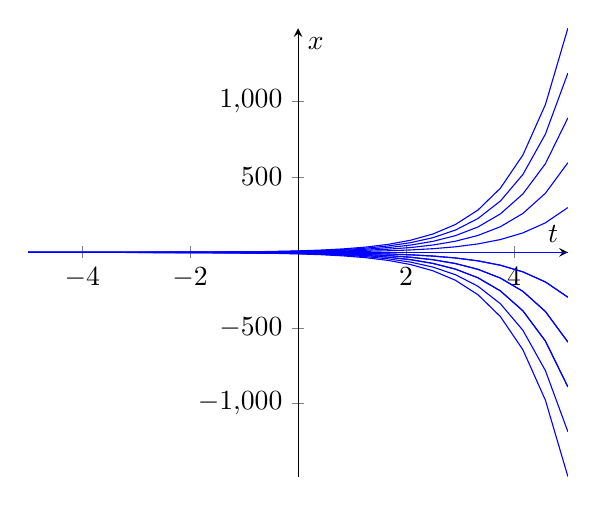
\begin{tikzpicture}
                    \begin{axis}[axis lines = middle, xlabel=$t$, ylabel=$x$]
                    
                    \foreach \C in {-10, -8, ..., 0, ..., 8, 10}
                    {
                    \addplot[color=blue]{\C * exp(x)};
                    }
                    \end{axis}
                    \end{tikzpicture}
                    \end{center}

                    \item For both $t > 0$ and $t < 0$, a solution always exists.

                    \item A solution is unique everywhere it exists.

                    \item \underline{$t > 0, x > 0$}: A solution exists provided $x > 0$. There is no condition $u(0,t) = g(t)$ to give a solution to this area otherwise.\\
                    \underline{$t > 0, x < 0$}: A solution exists provided $x < 0$. There is no condition $u(0,t) = g(t)$ to give a solution to this area otherwise.

                    \item \underline{$t < 0, x > 0$}: A solution exists provided $x > 0$. There is no condition $u(0,t) = g(t)$ to give a solution to this area otherwise.\\
                    \underline{$t < 0, x < 0$}: A solution exists provided $x < 0$. There is no condition $u(0,t) = g(t)$ to give a solution to this area otherwise.
                \end{enumerate}
			
			\item \begin{enumerate}[a)]
                    \item With the method of characteristics, we find
                    \begin{align*}
                        \frac{dt}{1} &= \frac{dx}{tx}\\
                        \int t\, dt &= \int \frac{dx}{x}\\
                        \frac{1}{2}t^2 &= \ln{\left(\frac{x}{C}\right)}\\
                        C\,e^{\frac{t^2}{2}} &= x
                    \end{align*}
                    Assuming $u(x,0) = f(x)$, we can find the solution to the PDE, which is $\boxed{u(x,t)=f\left(C\right)=f\left(xe^{-\frac{t^2}{2}}\right)}$. This create these characteristic curves:

                    \begin{center}
                    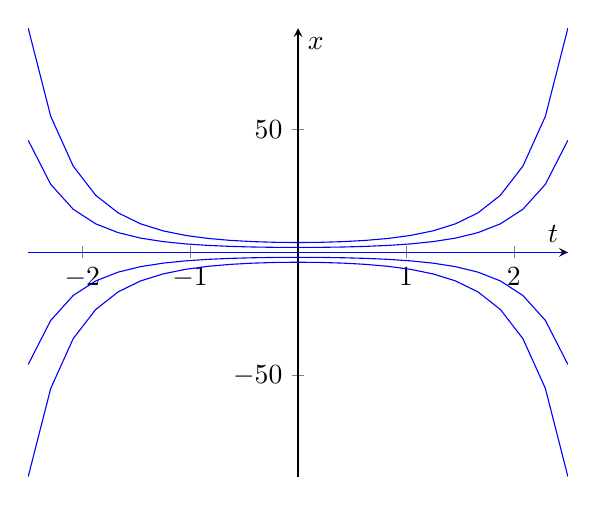
\begin{tikzpicture}
                    \begin{axis}[axis lines = middle, xlabel=$t$, ylabel=$x$]
                    
                    \foreach \C in {-4,-2,...,2,4}
                    {
                   \addplot[color=blue, domain=-2.5:2.5]{\C*exp(x^2/2)};
                   }
                    \end{axis}
                    \end{tikzpicture}
                    \end{center}
                    
                    \item For both $t > 0$ and $t < 0$ for $x \in \R$, the solution always exists.

                    \item The solution is uniquely determined everywhere it exists.

                    \item For both \underline{$t > 0, x > 0$} and \underline{$t > 0, x < 0$}, the solution is defined since there is an $x$ value that the characteristic curve can trace back to.

                    \item For the quadrants that satisfy \underline{$t < 0, x > 0$} and \underline{$t < 0, x < 0$}, the solution is also defined everywhere.
                \end{enumerate}
			
			\item \begin{enumerate}[a)]
                    \item By the method of characteristics,   
                    \begin{align*}
                        \frac{dt}{1} &= \frac{dx}{x^2}\\
                        t &= \frac{-1}{x} + C\\
                        t + \frac{1}{x} &= C\\
                    \end{align*}
                    This means that the equation for this PDE is $\boxed{u(x,t)=f\left(C\right)=f\left(t + \frac{1}{x}\right)}$, whose characteristic curves are:

                    \begin{figure}[H]
                        \centering
                        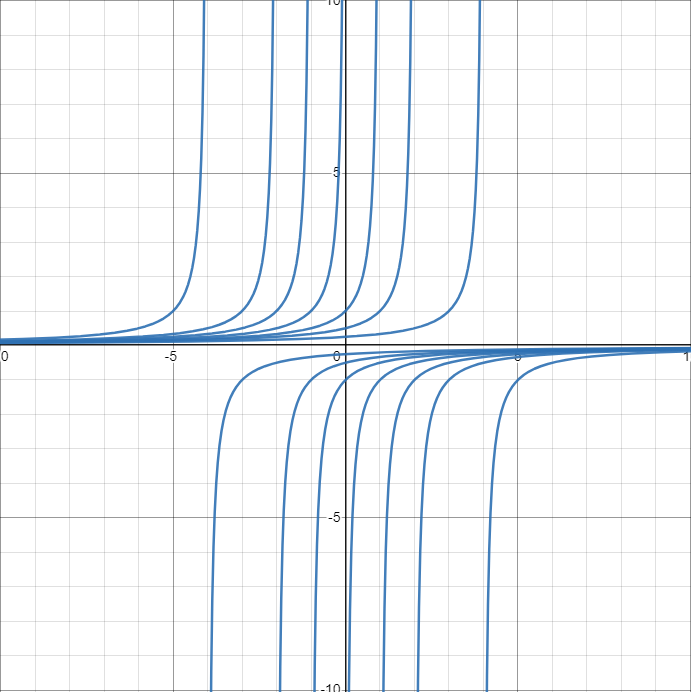
\includegraphics[width=2.3in]{7 graph.png}
                    \end{figure}
                    
                    \item For all $t > 0$ and $t < 0$, a solution exists for all $t\neq -\frac{1}{x}$.

                    \item Every solution that exists is unique.

                    \item \underline{$t > 0, x > 0$}: Solutions exist for all $t > 0$, $x > 0$.\\
                    
                    \underline{$t > 0, x < 0$}: There are solutions everywhere except for when $t = -\frac{1}{x}$ (when $C=0$). However, since this graph does not cross the $t$-axis anywhere, imposing a condition $u(0,t)=g(t)$ would not help.

                    \item \underline{$t < 0, x > 0$}: By symmetry, this case is the same as when $t > 0$, $x < 0$.\\
                    
                    \underline{$t < 0, x < 0$}: By symmetry, this case is the same as when $t > 0$, $x > 0$.
                \end{enumerate}
			
			\item \begin{enumerate}[a)]
                    \item Using the method of characteristics, we get the following:
                    \begin{align*}
                        \frac{dt}{1} &= \frac{dx}{x^2+1}\\
                        \int dt &= \int \frac{dx}{x^2+1}\\
                        t &= \arctan{(x)}+C\\
                        t - \arctan{(x)} &= C\\
                    \end{align*}
                    If we assume an initial condition $u(x,0) = f(x)$, then since the function is constant along characteristic curves, we have that $\boxed{u(x,t) = f(C) = f\left(t - \arctan{(x)}\right)}$. It has the following characteristic curves:
                    
                    \begin{center}
                    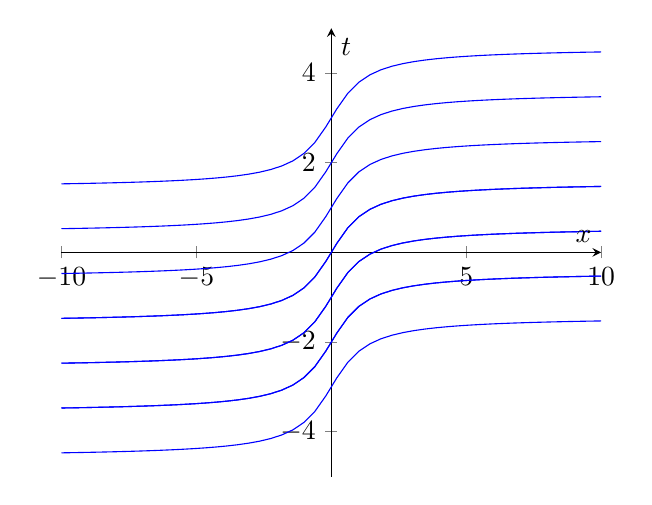
\begin{tikzpicture}
                    \begin{axis}[axis lines = middle, xlabel=$x$, ylabel=$t$, samples = 50, xmin=-10, xmax=10, ymin=-5, ymax=5]
                    
                    \foreach \C in {-3,...,0,..., 3}
                    {
                    \addplot[color=blue, domain=-10:10]{rad(atan(x)) + \C};
                    }
                    \end{axis}
                    \end{tikzpicture}
                    \end{center}
                    
                    \item \underline{$t > 0$}: A solution exists only when $0 < t < \arctan(x) + \frac{\pi}{2}$. There are no conditions $f(x)$ could satisfy to change this. A condition $u(0,t) = g(t)$ would be required.\\
                    \underline{$t < 0$}: A solution exists only when $\arctan(x) - \frac{\pi}{2} < t < 0$. There are no conditions $f(x)$ could satisfy to change this. A condition $u(0,t) = g(t)$ would be required.

                    \item The solution is uniquely determined everywhere it exists.

                    \item \underline{$t > 0, x > 0$}: Since we are only considering the upper-right quadrant, we must impose a condition $u(0,t) = g(t)$ when $t > \arctan(x)$. We also have that $u(x,t) = g(C)$. Taking $f(0) = g(0)$ and $f,g\in C^1$, we have our overall solution that
                    \begin{equation*}
                    u(x,t) =
                    \begin{cases}
                        f\left(t-\arctan(x)\right), & t < \arctan(x)\\
                        g\left(t-\arctan(x)\right), & t > \arctan(x)
                    \end{cases}
                    \end{equation*}
                    \underline{$t > 0, x < 0$}: Since we are only considering the lower-right quadrant, we must impose a condition $u(0,t) = g(t)$ when $t \leq \arctan(x) - \frac{\pi}{2}$. We also have that $u(x,t) = g(C)$. Taking $f(0) = g(0)$ and $f,g\in C^1$, we have our overall solution that
                    \begin{equation*}
                    u(x,t) =
                    \begin{cases}
                        f\left(t-\arctan(x)\right), & t > \arctan(x) - \frac{\pi}{2}\\
                        g\left(t-\arctan(x)\right), & t \leq \arctan(x) - \frac{\pi}{2}
                    \end{cases}
                    \end{equation*}

                    \item \underline{$t < 0, x > 0$}: Since we are only considering the upper-left quadrant, we must impose a condition $u(0,t) = g(t)$ when $t \geq \arctan(x) + \frac{\pi}{2}$. We also have that $u(x,t) = g(C)$. Taking $f(0) = g(0)$ and $f,g\in C^1$, we have our overall solution that
                    \begin{equation*}
                    u(x,t) =
                    \begin{cases}
                        f\left(t-\arctan(x)\right), & t \geq \arctan(x) + \frac{\pi}{2}\\
                        g\left(t-\arctan(x)\right), & t < \arctan(x) + \frac{\pi}{2}
                    \end{cases}
                    \end{equation*}
                    
                    \underline{$t < 0, x < 0$}: Since we are only considering the upper-right quadrant, we must impose a condition $u(0,t) = g(t)$ when $t < \arctan(x)$. We also have that $u(x,t) = g(C)$. Taking $f(0) = g(0)$ and $f,g\in C^1$, we have our overall solution that
                    \begin{equation*}
                    u(x,t) =
                    \begin{cases}
                        f\left(t-\arctan(x)\right), & t \geq \arctan(x)\\
                        g\left(t-\arctan(x)\right), & t < \arctan(x)
                    \end{cases}
                    \end{equation*}
                \end{enumerate}
			
			\item \begin{enumerate}[a)]
                    \item Using the method of characteristics, we get the following:

                    \begin{align*}\frac{dt}{1} &= \frac{dx}{t^2+1}\\
                        \int dt &= \int \frac{dx}{t^2+1}\\
                        \int (t^2 + 1)\,dt &= \int \,dx\\
			\frac{t^3}{3} + t + C &= x
                    \end{align*}

                    If we assume an initial condition $u(x,0) = f(x)$, then since the function is constant along characteristic curves, we have that $\boxed{u(x,t) = f(C) = f\left(x - \frac{t^3}{3} - t\right)}$. It has the following characteristic curves:
                   
                    \begin{figure}[H]
                        \centering
                        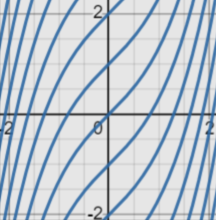
\includegraphics[width=2.3in]{9 graph.png}
                    \end{figure}

                    
                    \item The solution exists everywhere.

                    \item The solution is unique everywhere.

                    \item $t > 0, x > 0$: this is defined when C $\leq 0$. For a solution to be defined everywhere we need to impose on additional condition $u(t, 0) = g(t)$ that follow the same characteristic curves.

                    \item $t > 0, x < 0$: This solution is defined everywhere.\\ $t<0, x>0$: by symmetry, same as when $t>0, x<0$.\\$t<0, x<0$: by symmetry, same as when $t>0, x >0.$
                \end{enumerate}
			
			\item \begin{enumerate}[a)]
                    \item By the method of characteristics,
                    \begin{align*}
                        \frac{dt}{x+1} &= \frac{dx}{1}\\
                        \int (x+1)\,dx &= \int dt\\
                        \frac{1}{2}x^2 + x + C &= t\\
                        C &= t -\frac{1}{2}x^2 - x\\
                    \end{align*}
                    Assuming an initial condition $u(x, 0) = f(x)$, we can find the solution to the PDE. This turns out to be $\boxed{u(x,t) = f(C) = f\left(t - \frac{1}{2}x^2 - x\right)}$. Its characteristic curves are:
                    \begin{figure}[H]
                        \centering
                        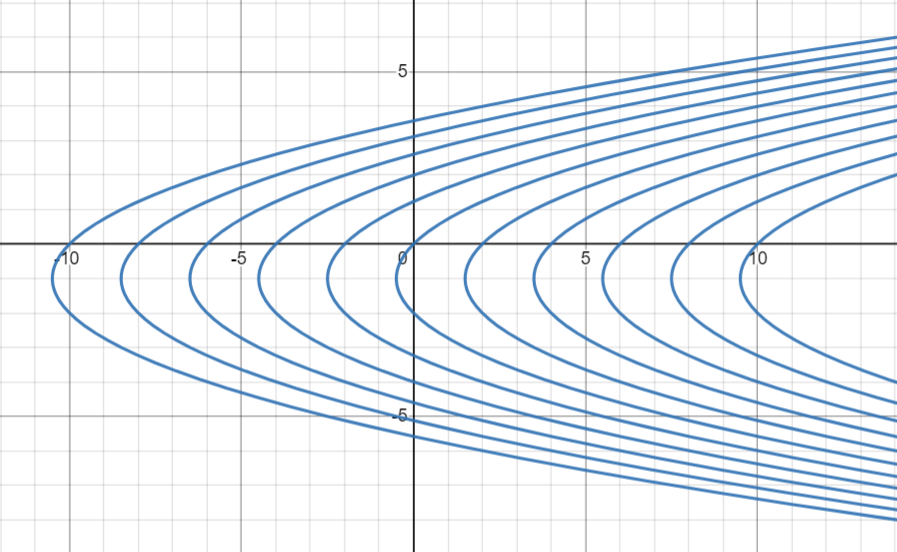
\includegraphics[height=2.3in]{10 graph.png}
                    \end{figure}
                    
                    \item The graph shows that not all characteristic curves will trace to a value of $x$. Notably, if $t < 0$, a solution always exists, but if $t > 0$, the solution does not necessarily exist.

                    \item Wherever the solution does exist, it appears it is not uniquely determined. Therefore, the solution is not uniquely determined anywhere.

                    \item \underline{$t > 0, x > 0$}: The solution is only defined on $t \leq \frac{1}{2}x^2 + x$. For $t > \frac{1}{2}x^2 + x$, we need to impose a condition at $x = 0$:
                    \begin{equation*}
                    u(x,t) =
                    \begin{cases}
                        f\left(t-\frac{1}{2}x^2 - x\right), & t \leq \frac{1}{2}x^2 + x\\
                        g\left(t-\frac{1}{2}x^2 - x\right), & t > \frac{1}{2}x^2 + x
                    \end{cases}
                    \end{equation*}\\
                    \underline{$t > 0, x < 0$}: In the same way, we need to impose a condition at $x = 0$ since the solution is not defined when $t > \frac{1}{2}x^2 + x+\frac{1}{2}$:
                    \begin{equation*}
                    u(x,t) =
                    \begin{cases}
                        f\left(t-\frac{1}{2}x^2 - x\right), & t \leq \frac{1}{2}x^2 + x + \frac{1}{2}\\
                        g\left(t-\frac{1}{2}x^2 - x\right), & t > \frac{1}{2}x^2 + x + \frac{1}{2}
                    \end{cases}
                    \end{equation*}

                    \item \underline{$t < 0, x > 0$}: The solution is defined everywhere for this quadrant.\\
                    \underline{$t < 0, x < 0$}: An $x$-value can be traced back to a characteristic curve in this quadrant, so the solution is defined everywhere for this quadrant.
                \end{enumerate}

                \item \begin{enumerate}[a)]
                    \item Using the method of characteristics, we get the following:

                    \begin{align*}\frac{dt}{(x+1)^2} &= \frac{dx}{1}\\
                        \int dt &= \int (x+1)^2 dx\\
                        t &= \frac{(x + 1)^3}{3} + C\\
                    \end{align*}

                    If we assume an initial condition $u(x,0) = f(x)$, then since the function is constant along characteristic curves, we have that $\boxed{u(x,t) = f(C) = f\left(t - \frac{(x+1)^3}{3}\right)}$. It has the following characteristic curves:
                   
                    \begin{figure}[H]
                        \centering
                        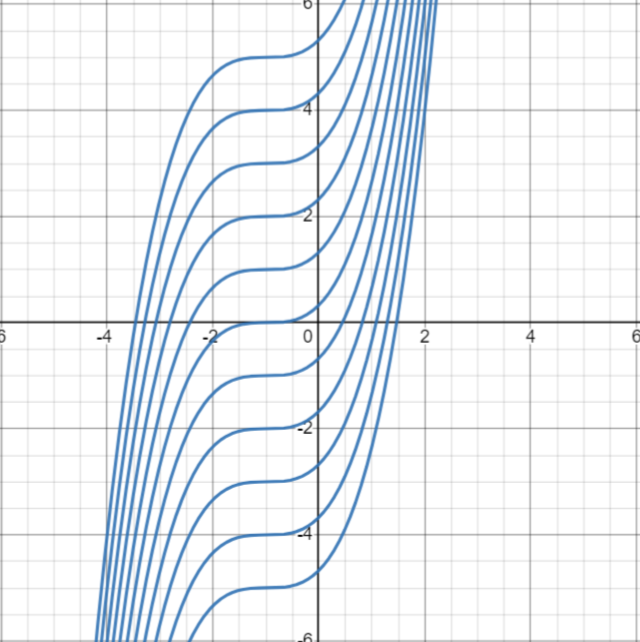
\includegraphics[width=2.3in]{11 graph.png}
			
                    \end{figure}

                    
                    \item The solution exists everywhere.

                    \item The solution is unique everywhere.

                    \item $t > 0, x > 0$: this is defined when C $\leq 0$. For a solution to be defined everywhere we need to impose on additional condition $u(t, 0) = g(t)$ that follow the same characteristic curves.

                    \item $t > 0, x < 0$: This solution is defined everywhere.\\ $t<0, x>0$: by symmetry, same as when $t>0, x<0$.\\$t<0, x<0$: by symmetry, same as when $t>0, x >0.$

                \end{enumerate}

                \item \begin{enumerate}[a)]
                    \item With the method of characteristics, we are able to find that
                    \begin{align*}
                        \frac{dt}{x^2+1} &= \frac{dx}{1}\\
                        \int dt &= \int (x^2+1)\,dx\\
                        t = \frac{x^3}{3} + x + C
                    \end{align*}
                    IF we assume $u(0, x) = f(x)$, we find that $\boxed{u(x,t) = f(C) = f\left(t - \frac{x^3}{3} - x\right)}$. This yields the characteristic curves.
                    \begin{figure}[H]
                        \centering
                        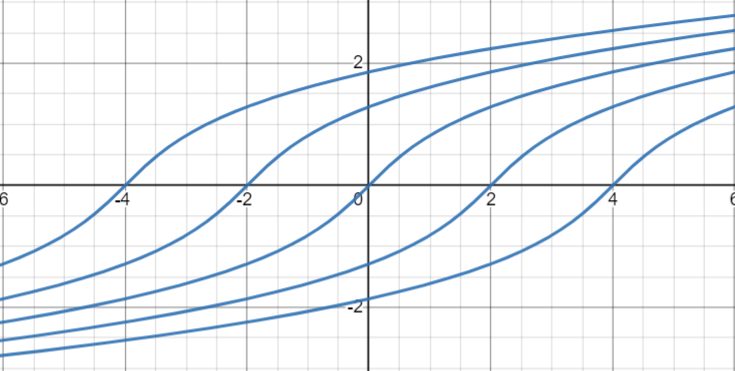
\includegraphics[height=2.3 in]{12 graph.png}
                    \end{figure}
                    
                    \item Across all values of $x$ and assuming $u(0,x)=f(x)$, we find that the solution exists for positive and negative values of $t$.

                    \item The solution is uniquely determined for both cases $t > 0$ and $t < 0$.

                    \item \underline{$t > 0$, $x > 0$}: We have a solution for all $t\geq \frac{x^3}{3}$, but for $t < \frac{x^3}{3}$, we have to impose an additional condition $u(t,0) = g(t)$, taking $f(0)=g(0)$ and $f,g\in C^1$. This gives us the solution that \begin{equation*}
                    u(x,t) =
                    \begin{cases}
                        f\left(t - \frac{x^3}{3} - x\right), & t \geq \frac{x^3}{3} + x\\
                        g\left(t - \frac{x^3}{3} - x\right), & t < \frac{x^3}{3} + x
                    \end{cases}
                    \end{equation*}\\
                    \underline{$t > 0$, $x < 0$}: A solution exists everywhere in this quadrant.
                    

                    \item \underline{$t < 0$, $x > 0$} By symmetry to $t > 0$, $x < 0$, a solution exists everywhere in this quadrant.\\
                    \underline{$t < 0$, $x < 0$}: We have a solution for all $t \leq  \frac{x^3}{3}$, but for $t > \frac{x^3}{3}$, we have to impose an additional condition $u(t,0) = g(t)$, taking $f(0)=g(0)$ and $f,g\in C^1$. This gives us the solution that \begin{equation*}
                    u(x,t) =
                    \begin{cases}
                        f\left(t - \frac{x^3}{3} - x\right), & t \leq \frac{x^3}{3} + x\\
                        g\left(t - \frac{x^3}{3} - x\right), & t > \frac{x^3}{3} + x
                    \end{cases}
                    \end{equation*}
                \end{enumerate}

                \item \begin{enumerate}[a)]
                    \item By the method of characteristics:
                    \begin{align*}
                        \frac{dt}{x^2-1} &= \frac{dx}{1}\\
                        \int (x^2-1)\,dx &= \int dt\\
                        \frac{1}{3}x^3 - x + C &= t\\
                        C &= t - \frac{1}{3}x^3 + x
                    \end{align*}
                    Taking an initial condition $u(x, 0) = f(x)$, we find that $\boxed{u(x,t) = f(C) = f\left(t - \frac{x^3}{3} + x\right)}$, whose characteristic lines are:
                    \begin{figure}[H]
                        \centering
                        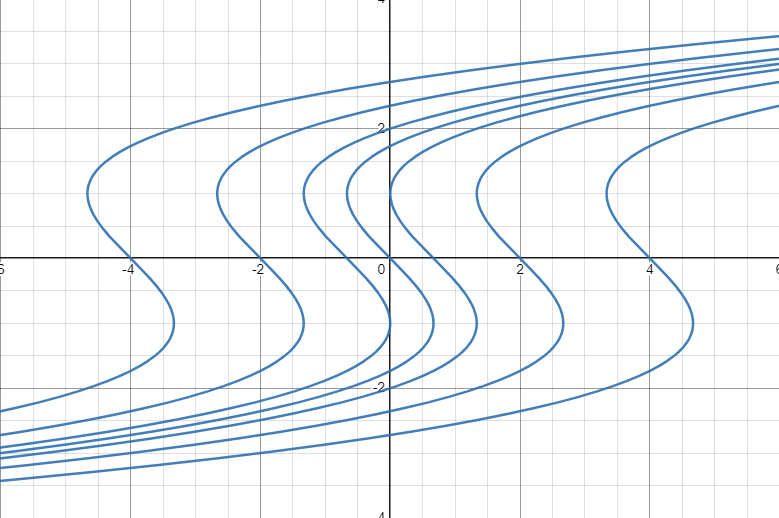
\includegraphics[width=2.3 in]{13 graph.png}
                    \end{figure}
                    
                    \item For $x \in \R$, the solution exists for both $t > 0$ and $t < 0$.

                    \item For $t > 0$, the solution is uniquely determined for $t > \frac{1}{3}x^3 - x + \frac{2}{3}$. For $t < 0$, the solution is uniquely determined for $t < \frac{1}{3}x^3 - x - \frac{2}{3}$.

                    \item \underline{$t > 0, x > 0$}: The solution is only defined if $t \leq \frac{1}{3}x^3 - x + \frac{2}{3}$. Otherwise, a boundary has to be defined at $x = 0$,
                    \begin{equation*}
                    u(x,t) =
                    \begin{cases}
                        f\left(t - \frac{x^3}{3} + x\right), & t \leq \frac{x^3}{3} - x + \frac{2}{3}\\
                        g\left(t - \frac{x^3}{3} + x\right), & t > \frac{x^3}{3} - x + \frac{2}{3}
                    \end{cases}
                    \end{equation*}
                    \underline{$t > 0, x < 0$}: The solution is only defined if $t \geq \frac{1}{3}x^3 - x - \frac{2}{3}$. Otherwise, a boundary has to be defined at $x = 0$,
                    \begin{equation*}
                    u(x,t) =
                    \begin{cases}
                        f\left(t - \frac{x^3}{3} + x\right), & t \geq \frac{x^3}{3} - x - \frac{2}{3}\\
                        g\left(t - \frac{x^3}{3} + x\right), & t < \frac{x^3}{3} - x - \frac{2}{3}
                    \end{cases}
                    \end{equation*}

                    \item \underline{$t < 0, x > 0$}: The solution is only defined if $t \leq \frac{1}{3}x^3 - x  \frac{2}{3}$. Otherwise, a boundary has to be defined at $x = 0$,
                    \begin{equation*}
                    u(x,t) =
                    \begin{cases}
                        f\left(t - \frac{x^3}{3} + x\right), & t \leq \frac{x^3}{3} - x + \frac{2}{3}\\
                        g\left(t - \frac{x^3}{3} + x\right), & t > \frac{x^3}{3} - x + \frac{2}{3}
                    \end{cases}
                    \end{equation*}\\
                    \underline{$t < 0, x < 0$}: The solution is only defined if $t \geq \frac{1}{3}x^3 - x - \frac{2}{3}$. Otherwise, a boundary has to be defined at $x = 0$,
                    \begin{equation*}
                    u(x,t) =
                    \begin{cases}
                        f\left(t - \frac{x^3}{3} + x\right), & t \geq \frac{x^3}{3} - x - \frac{2}{3}\\
                        g\left(t - \frac{x^3}{3} + x\right), & t < \frac{x^3}{3} - x - \frac{2}{3}
                    \end{cases}
                    \end{equation*}
                \end{enumerate}
		\end{enumerate}
		
	\end{ans}
	\begin{boldenv}
		\underline{Problem 2}. \begin{enumerate}[a)]
		    \item Find the general solution to each of the following equations
      \begin{enumerate}[start=14, resume*=problems]
			\item $xu_x + yu_y = 0$
            \item $xu_x - yu_y = 0$
		\end{enumerate}
        in $\{(x,y)\neq (0,0)\}$; when is this solution continuous at $(0,0)$ Explain the difference between these two cases.

        \item Find the general solution to each of the following equations
      \begin{enumerate}[start=16, resume*=problems]
			\item $yu_x + xu_y = 0$
            \item $yu_x - xu_y = 0$
		\end{enumerate}
        in $\{(x,y)\neq (0,0)\}$; when is this solution continuous at $(0,0)$ Explain the difference between these two cases.
		\end{enumerate}
	\end{boldenv}
	
	\begin{ans}
		\begin{enumerate}[resume*=answers]
			\item
		\begin{align*}xu_x + yu_y &= 0\\
				\frac{dx}{x} &= \frac{dy}{y} \\
				\ln|x| + C_1 &= \ln|y| \\
				C_2x -y \\
				C_2 &= \frac{y}{x} \\
			so, u(x, y) &= f(C) \\
			\Aboxed{u(x, y) &= f(\frac{y}{x})} \\ \end{align*}

		\begin{figure}[H]
                        \centering
                        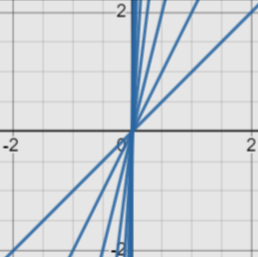
\includegraphics[width=2.3in]{14 graph.png}

                    \end{figure}
			
			\item \begin{align*}xu_x + yu_y &= 0\\
				\frac{dx}{x} &= \frac{dy}{y} \\
				\ln|x| &= \ln|(\frac{y}{C})^{-1}| \\
				x &= \frac{c}{y}\\
				y &= \frac{c}{x}\\
				u(0, y) &= f(y) \\
				f \in C'\\
			\Aboxed{u(x, y) &= f(C) = f(yx)} \\ \end{align*}

		\begin{figure}[H]
                        \centering
                        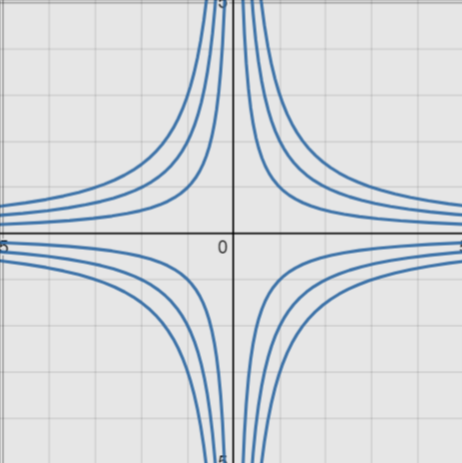
\includegraphics[width=2.3in]{15 graph.png}

                    \end{figure}

                After observing both graphs, the former equation is continuous at the origin only if the function $u(x,y) = f(\frac{x}{y})$ is a constant. The only condition for the latter equation to be continuous at $(0,0)$ is $f \in C^1$.
			
			\item \textbf{\emph{Discussion of when the solution is continuous at the origin after the graph of problem 17.}}\\
            By the method of characteristics,
            \begin{align*}
                \frac{dx}{y} &= \frac{dy}{x}\\
                \int x\,dx &= \int y\,dy\\
                \frac{1}{2}x^2 + C &= \frac{1}{2}y^2\\
                x^2 + C &= y^2\\
                C &= y^2 - x^2\\
            \end{align*}
			Therefore, $u(x,y) = f(C) = f(y^2 - x^2)$, which looks like this:\\
            \begin{figure}[H]
                \centering
                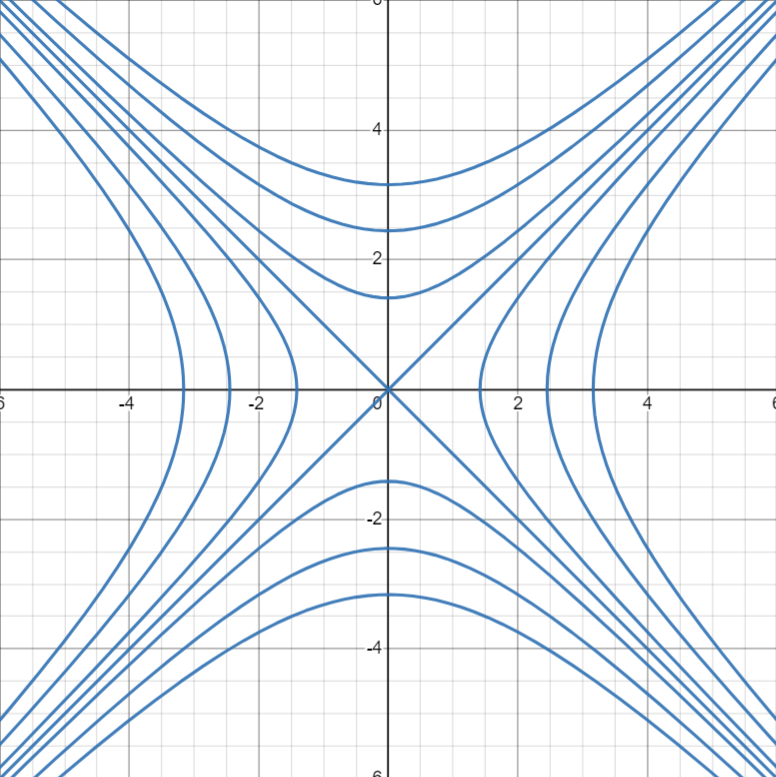
\includegraphics[width=2.3 in]{16 graph.png}
            \end{figure}
            
			\item We can do the same process we did in problem 16. This will result in
            \begin{align*}
                \frac{dx}{y} &= \frac{dy}{-x}\\
                \int x\,dx &= -\int y\,dy\\
                \frac{1}{2}x^2 + C &= -\frac{1}{2}y^2\\
                x^2 + C &= -y^2\\
                C &= x^2 + y^2\\
            \end{align*}
            The resulting solution (graph below) is $u(x,y) = f(C) = f(x^2 + y^2)$.\\
            \begin{center}
            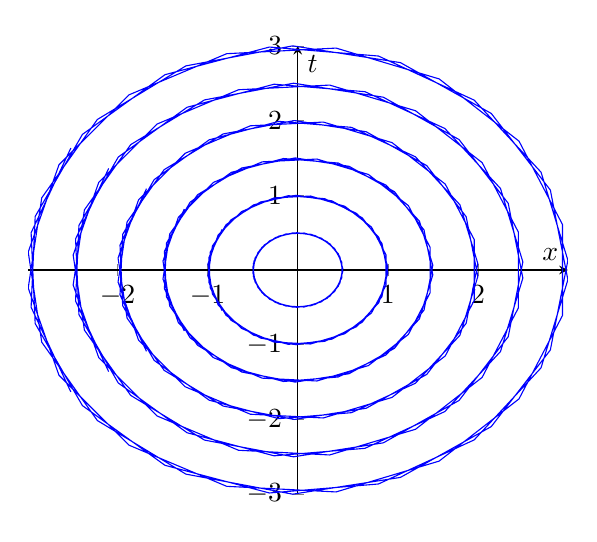
\begin{tikzpicture}
            \begin{axis}[axis lines = middle, xlabel=$x$, ylabel=$t$, samples = 50]
                    
                    \foreach \C in {0,0.5,..., 2.5,3}
                    {
                    \addplot[color=blue, domain=-10:10]({\C * cos(deg(x))}, {\C * sin(deg(x))});
                    }
                
            \end{axis}
            \end{tikzpicture}
            \end{center}

            After looking at both graphs, both appear to be continuous at the origin if $f(0)$ is well-defined (which it is since we also assume $f \in C^1$).
			
		\end{enumerate}
	\end{ans}
	
	\begin{boldenv}
		\underline{Problem 3}. In the same way consider equations:
		\begin{enumerate}[(1), start=18, series=problems]
			\item $(x^2+1)yu_x + (y^2+1)xu_y = 0$
			\item $(x^2+1)yu_x - (y^2+1)xu_y = 0$
		\end{enumerate}
	\end{boldenv}
	
	\begin{ans}
		\begin{enumerate}[resume*=answers]
			\item We find the characteristic curves via the following:
            \begin{align*}
                \frac{dx}{(x^2+1)y} &= \frac{dy}{(y^2+1)x}\\
                \int \frac{x}{(x^2+1)}dx &= \int\frac{y}{(y^2+1)}dy\\
                \frac{1}{2}\ln|x^2+1| + C_1 &= \frac{1}{2}\ln|y^2+1|\\
                \ln|x^2+1| + C_2 &= \ln|y^2+1|\\
                C(x^2+1) &= y^2+1 \tag{letting $C = e^{C_2}$}\\
                C &= \frac{y^2+1}{x^2+1}
            \end{align*}
            We take $u(0,y) = f(y)$, and since $u$ is constant along the characteristic curves, that means that
            \[\boxed{u(x,y) = f(C) = f\left(\frac{y^2+1}{x^2+1}\right)}\]
            The graph of the characteristic curves looks like this:
            \begin{figure}[H]
                \centering
                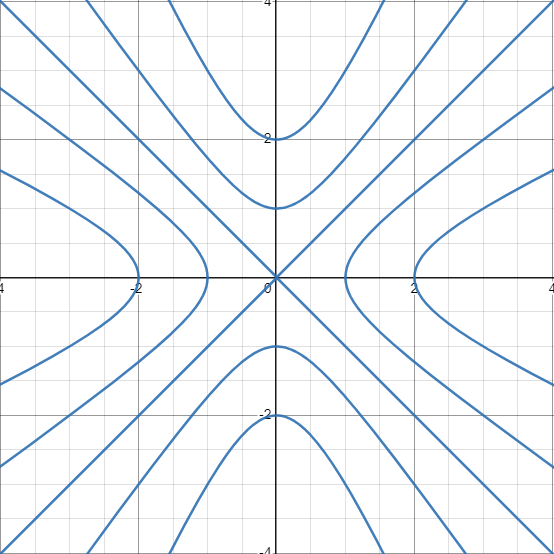
\includegraphics[width=2.3in]{18 graph.png}
            \end{figure}
            Since we take $f\in C^1$, and $\frac{y^2+1}{x^2+1}$ is continuous everywhere, that means that the solution is continuous everywhere it exists (when $C > 0$), including at $(0,0)$.
            
			\item We find the characteristic curves via the following:
            \begin{align*}
                \frac{dx}{(x^2+1)y} &= -\frac{dy}{(y^2+1)x}\\
                -\int \frac{x}{(x^2+1)}dx &= \int\frac{y}{(y^2+1)}dy\\
                -\frac{1}{2}\ln|x^2+1| + C_1 &= \frac{1}{2}\ln|y^2+1|\\
                C_2 - \ln|x^2+1| &= \ln|y^2+1|\\
                C(x^2+1)^{-1} &= y^2+1 \tag{letting $C = e^{C_2}$}\\
                C &= (y^2+1)(x^2+1)
            \end{align*}
            We take $u(0,y) = f(y)$, and since $u$ is constant along the characteristic curves, that means that
            \[\boxed{u(x,y) = f(C) = f\left((y^2+1)(x^2+1)\right)}\]
            The graph of the characteristic curves looks like this:
            \begin{figure}[H]
                \centering
                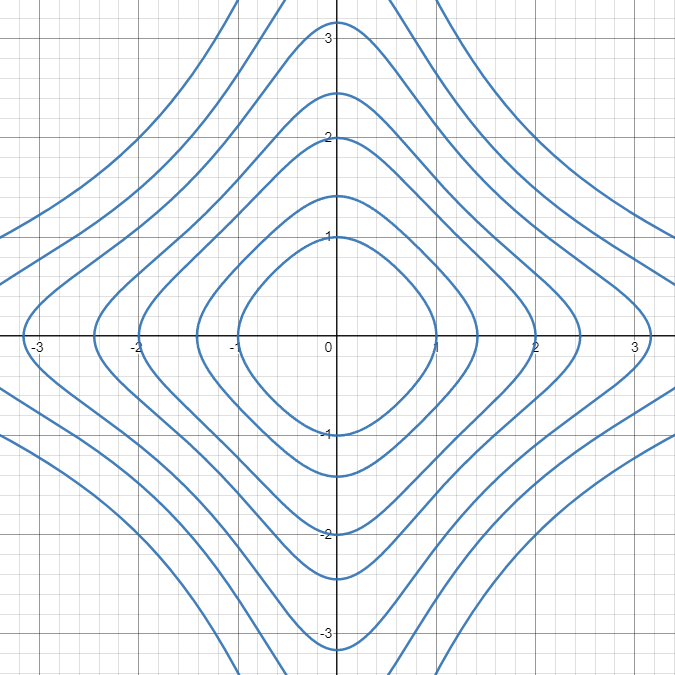
\includegraphics[width=2.3in]{19 graph.png}
            \end{figure}
            Since we take $f\in C^1$, and $(y^2+1)(x^2+1)$ is continuous everywhere, that means that the solution is continuous everywhere it exists (when $C \geq 1$), including at $(0,0)$.\\

            
		\end{enumerate}
	\end{ans}
	
	\begin{boldenv}
		\underline{Problem 4}. Find the solutions of
		\begin{enumerate}[resume*=problems]
			\item $\begin{cases}
			    u_x + 3u_y = xy,\\
                u|_{x=0} = 0
			\end{cases}$
			\item $\begin{cases}
			    u_x + 3u_y = u,\\
                u|_{x=0} = 0
			\end{cases}$
		\end{enumerate}
	\end{boldenv}
	
	\begin{ans}
		\begin{enumerate}[resume*=answers]
			\item As usual, we find the integral curves via the method of characteristics.
                \[\frac{dx}{1} = \frac{dy}{3} = \frac{du}{xy}.\]
                We begin by working with the $dx$ and $dy$ parts.
                \begin{align*}
                    \frac{dx}{1} &= \frac{dy}{3}\\
                    \int 3\,dx &= \int dy\\
                    3x + C_1 &= y\\
                    C_1 &= y - 3x
                \end{align*}
                Now we look at the $dx$ and $du$ parts.
                \begin{align*}
                    \frac{dx}{1} &= \frac{du}{xy}\\
                    \int xy\,dx &= \int du\\
                    \int x(3x+C_1)\,dx &= \int du\tag{substituting for $y$}\\
                    \int (3x^2 + C_1x)\,dx &= \int du\\
                    x^3 + \frac{1}{2}C_1x^2 + C_2 &= u
                \end{align*}
			    We can now let $C_2 = f(C_1)$ to get our general solution that
                \[u(x,y) = x^3 + \frac{1}{2}C_1x^2 + f(C_1) = x^3 + \frac{1}{2}(y - 3x)x^2 + f(y - 3x).\]
                After that, we plug in our initial condition.
                \begin{equation*}
                    u(0,y) = f(y-3(0)) = 0\\
                    \implies f(y) = 0\\
                    \implies f(y-3x) = 0.
                \end{equation*}
                Taking this into account gives us our final solution of
                \[\boxed{u(x,y) = x^3 + \frac{1}{2}(y-3x)x^2}\]
                
			\item As usual, we find the integral curves via the method of characteristics.
                \[\frac{dx}{1} = \frac{dy}{3} = \frac{du}{xy}.\]
                We begin by working with the $dx$ and $dy$ parts.
                \begin{align*}
                    \frac{dx}{1} &= \frac{dy}{3}\\
                    \int 3\,dx &= \int dy\\
                    3x + C_1 &= y\\
                    C_1 &= y - 3x
                \end{align*}
                Now we look at the $dx$ and $du$ parts.
                \begin{align*}
                    \int \frac{dx}{1} &= \int \frac{du}{u}\\
                    \int xy\,dx &= \ln(\frac{u}{C_2})\\
                    u = C-2e^x (let c_2 = f(c_1))\\
                    u = f(y-3x)e^x\\
                    x^3 + \frac{1}{2}C_1x^2 + C_2 &= u
                \end{align*}

                \begin{equation*}
                    u(0,y) = f(y) = y\\
                    \implies f(y) = 0\\
                    \implies f(y-3x) = y-3x.
                \end{equation*}
                Taking this into account gives us our final solution of
                \[\boxed{u(x,y) = (y-3x)e^x}\]
			
		\end{enumerate}
	\end{ans}
	
	\begin{boldenv}
		\underline{Problem 5}. Find the general solutions to each of
		\begin{enumerate}[resume*=problems]
			\item $yu_x - xu_y = x$
			\item $yu_x - xu_y = x^2$
			\item $yu_x + xu_y = x$
			\item $yu_x + xu_y = x^2$
		\end{enumerate}
	\end{boldenv}
	
	\begin{ans}
		\begin{enumerate}[resume*=answers]
			\item First, let's find the integral curves via the method of characteristics:
                $$\frac{dx}{y} = -\frac{dy}{x} = \frac{du}{x}$$
            Now, let's find the solution using certain integral curves:
            \begin{align*}
                \frac{dx}{y} &= -\frac{dy}{x}\\
                \int x\,dx &= -\int y\,dy\\
                -\frac{1}{2}y^2 &= \frac{1}{2}x^2 + C\\
                -y^2 &= x^2 + C\\
                C &= x^2 + y^2
            \end{align*}
            Continuing this trend with another integral curve and subbing in $y$ as necessary:
            \begin{align*}
                \frac{dx}{y} &= \frac{du}{x}\\
                \int \frac{x}{\sqrt{C-x^2}} dx &= \int du
            \end{align*}
            The integral of $du$ is easy, so let's specify on the left-hand side of the integral:
                $$\int \frac{x}{\sqrt{C-x^2}} dx$$
			Let's use the following substitution and solve accordingly (bringing back the right-hand side while we're at it):
            \begin{align*}
                r &= C-x^2\\
                dr &= -2x dx\\
                -\frac{1}{2}\int r^{-1/2} dr &= \int du\\
                -\sqrt{r} + D &= u\\
                -\sqrt{C-x^2} + D &= u
            \end{align*}
            Now, letting $D = f(C) = f(x^2 + y^2)$, we can complete the integration. We find that our answer is $\boxed{u(x, y) = -\sqrt{C-x^2} + f(x^2 + y^2)}$\\
            
			\item First, let's find the integral curves via the method of characteristics:
                $$\frac{dx}{y} = -\frac{dy}{x} = \frac{du}{x^2}$$
            Now, let's find the solution using certain integral curves:
            \begin{align*}
                \frac{dx}{y} &= -\frac{dy}{x}\\
                \int x\,dx &= -\int y\,dy\\
                -\frac{1}{2}x^2 + C_1&= \frac{1}{2}x^2 + C_1\\
                -y^2 &= x^2 + C_2\\
                C_3 &= x^2 + y^2
            \end{align*}
            Continuing this trend with another integral curve and subbing in $x$ as necessary:
            \begin{align*}\frac{dy}{-x} &= \frac{du}{x^2}\\
                \int \sqrt{(C_3-y^2} dy &= \int du\\
		y &= \sqrt{C_3 }\sin\theta \\
		dy &= \sqrt{C_3} \cos d\theta \\
		\pm \sqrt{C_3 - C_3 \sin \theta}(\sqrt{C_3}cos\theta) &= du\\
		\pm C_3\cos\theta d\theta &= du\\
		\pm C_3 \int \frac{1 +cos\theta}{2} d\theta &= du\\
		\pm C_3 [\int \frac{d\theta}{2} + \int \frac{\cos(2\theta)}{2} d\theta] &= du\\
		\pm C_3 [\frac{\theta}{2} + \frac{1}{4}\sin(2\theta) + D] &= du\\
		\Aboxed{u(x, y) = \pm C_3[\frac{\arccos(\frac{y}{C_3})}{2} + \frac{1}{4}\sin(2 \arcsin (\frac{y}{\sqrt{C_3}}) + D]} \end{align*}
				
			\item We use the method of characteristics to get that
            \[\frac{dx}{y} = \frac{dy}{x} = \frac{du}{x}.\]
            We begin by working with the $dx$ and $dy$ parts of this equation.
            \begin{align*}
                \frac{dx}{y} &= \frac{dy}{x}\\
                x\, dx &= y\, dy\\
                \frac{1}{2}x^2 &= \frac{1}{2}y^2 + C \tag{after integrating}\\
                C &= \frac{1}{2}x^2 - \frac{1}{2}y^2
            \end{align*}
            Now shifting our focus to the $dy$ and $du$ parts of the equation gives us
            \begin{align*}
                \frac{dy}{x} &= \frac{du}{x}\\
                \int dy &= \int du\\
                y + D &= u
            \end{align*}
            $D$ is only constant with respect to $y$, so it is actually an arbitrary function. We will let this be an arbitrary function $\phi$ with respect to $C$. Now we have
            \begin{align*}
                u(x,y) &= y + D\\
                &= y + \phi(C)\\
                \Aboxed{u(x,y) &= y + \phi\left(\frac{1}{2}x^2 - \frac{1}{2}y^2\right)}
            \end{align*}
            
				
			\item Following the same process,
                $$\frac{dx}{y} = \frac{dy}{x} = \frac{du}{x^2}$$
            \begin{align*}
                \frac{dx}{y} &= \frac{dy}{x}\\
                \int x\,dx &= \int y\,dy\\
                \frac{1}{2}y^2 &= \frac{1}{2}x^2 + C_1\\
                y^2 &= x^2 + C_1\\
                x &= \sqrt{y^2 - C_1}
            \end{align*}
            Subbing in x when needed:
            \begin{align*}
                \frac{dy}{x} &= \frac{du}{x^2}\\
                \int x\,dy &= \int du\\
                \int \sqrt{y^2 - C_1}\,dy &= \int du
            \end{align*}
            Next, we use trig substitution and integration by parts on the left-hand side of the equation.
            \begin{align*}
                y &= \sqrt{C_1} \sec{(\theta)}\\
                dy &= \sqrt{C_1} \sec{(\theta)} \tan{(\theta)} d\theta\\
                \int du &= \int \sqrt{C_1 \sec^2{(\theta)} - C_1}\,(\sqrt{C_1}\sec{(\theta)}\tan{(\theta)}) d\theta\\
                \int du &= C_1\int \sec{(\theta)}\tan^2{(\theta)} d\theta\\
            \end{align*}
            Using
            \begin{align*}
            a &= \tan{(\theta)}\\
            da &= \sec^2{(\theta)}\\
            and\\
            dv &= \sec{(\theta)}\sec{(\theta)} d\theta\\
            v &= \sec{(\theta)}\\  
            \end{align*}
            We can rewrite the integral as:
            \begin{align*}
                \int du &= C_1\left( \int \sec{(\theta)}\tan{(\theta)} - \int \sec^3{(\theta)} d\theta \right)\\
                \int du &= C_1\left( \int \sec{(\theta)}\tan{(\theta)} - \int \sec{(\theta)}(1 + \tan^2{(\theta)})\,d\theta \right)\\
                \int du &= C_1\left( \int \sec{(\theta)}\tan{(\theta)} - \left( \int \sec{(\theta)}\,d\theta + \int \sec{(\theta)}\tan^2{(\theta)}\,d\theta\right) \right)\\
            \end{align*}
            It looks like the integral repeats! As such, we can rewrite this integral as
            \begin{align*}
                \int \sec{(\theta)}\tan^2{(\theta)} = \sec{(\theta)}\tan{(\theta)} - |\sec{(\theta)} + \sec{(\theta)}| - \int \sec{(\theta)}\tan^2{(\theta)} d\theta\\
                \int \sec{(\theta)}\tan^2{(\theta)} = \frac{\sec{(\theta)}\tan{(\theta)} - |\sec{(\theta)} + \sec{(\theta)}|}{2}\\
            \end{align*}
            Going back to our trig substitution, it looks as if, picturing a right triangle, the hypotenuse is $y$ and the adjacent side relative to the angle is $\sqrt{C_1}$. Following this, we can further simplify our answer to
            \begin{align*}
                u(x, y) = \frac{1}{2}\left( \frac{y\sqrt{y^2-C_1}}{C_1} - |\frac{y+\sqrt{y^2-C_1}}{\sqrt{C_1}} \right) + D
            \end{align*}
            Finally, assuming $D = f(C_1) = f(y^2 - x^2)$ as hinted by the first integral curve, the final answer is
            \begin{align*}
                \boxed{u(x, y) = \frac{1}{2}\left( \frac{y\sqrt{y^2-C_1}}{C_1} - |\frac{y+\sqrt{y^2-C_1}}{\sqrt{C_1}} \right) + f(y^2-x^2)}
            \end{align*}

{\color{red} You shouldn't have this constant $C_{1}$ in your solution, it should only be in terms of the variables $x$ and $y$. The same comment applies to the problem above. }
			\end{enumerate}
		\end{ans}
		
	\end{document} 
